% vim:ts=4:sw=4
% Copyright (c) 2014 Casper Ti. Vector
% Public domain.

\chapter{绪论}
% 中文测试文字。
\section{研究背景}
\subsection{高速公路交通研究背景}

高速公路网络已经成为支撑国家经济发展、服务群众生活、保障国家安全的战略资源和设施。截止2016年底,我国公路通车总里程达到457万公里,其中高速公路12万公里,2017年将新增4500公里,是世界上规模最大的高速公路网络(如图\ref{gaosugonglu}所示)。 

				\begin{figure}[h]
				\centering
						\begin{minipage}{0.8\linewidth}
							\centering
							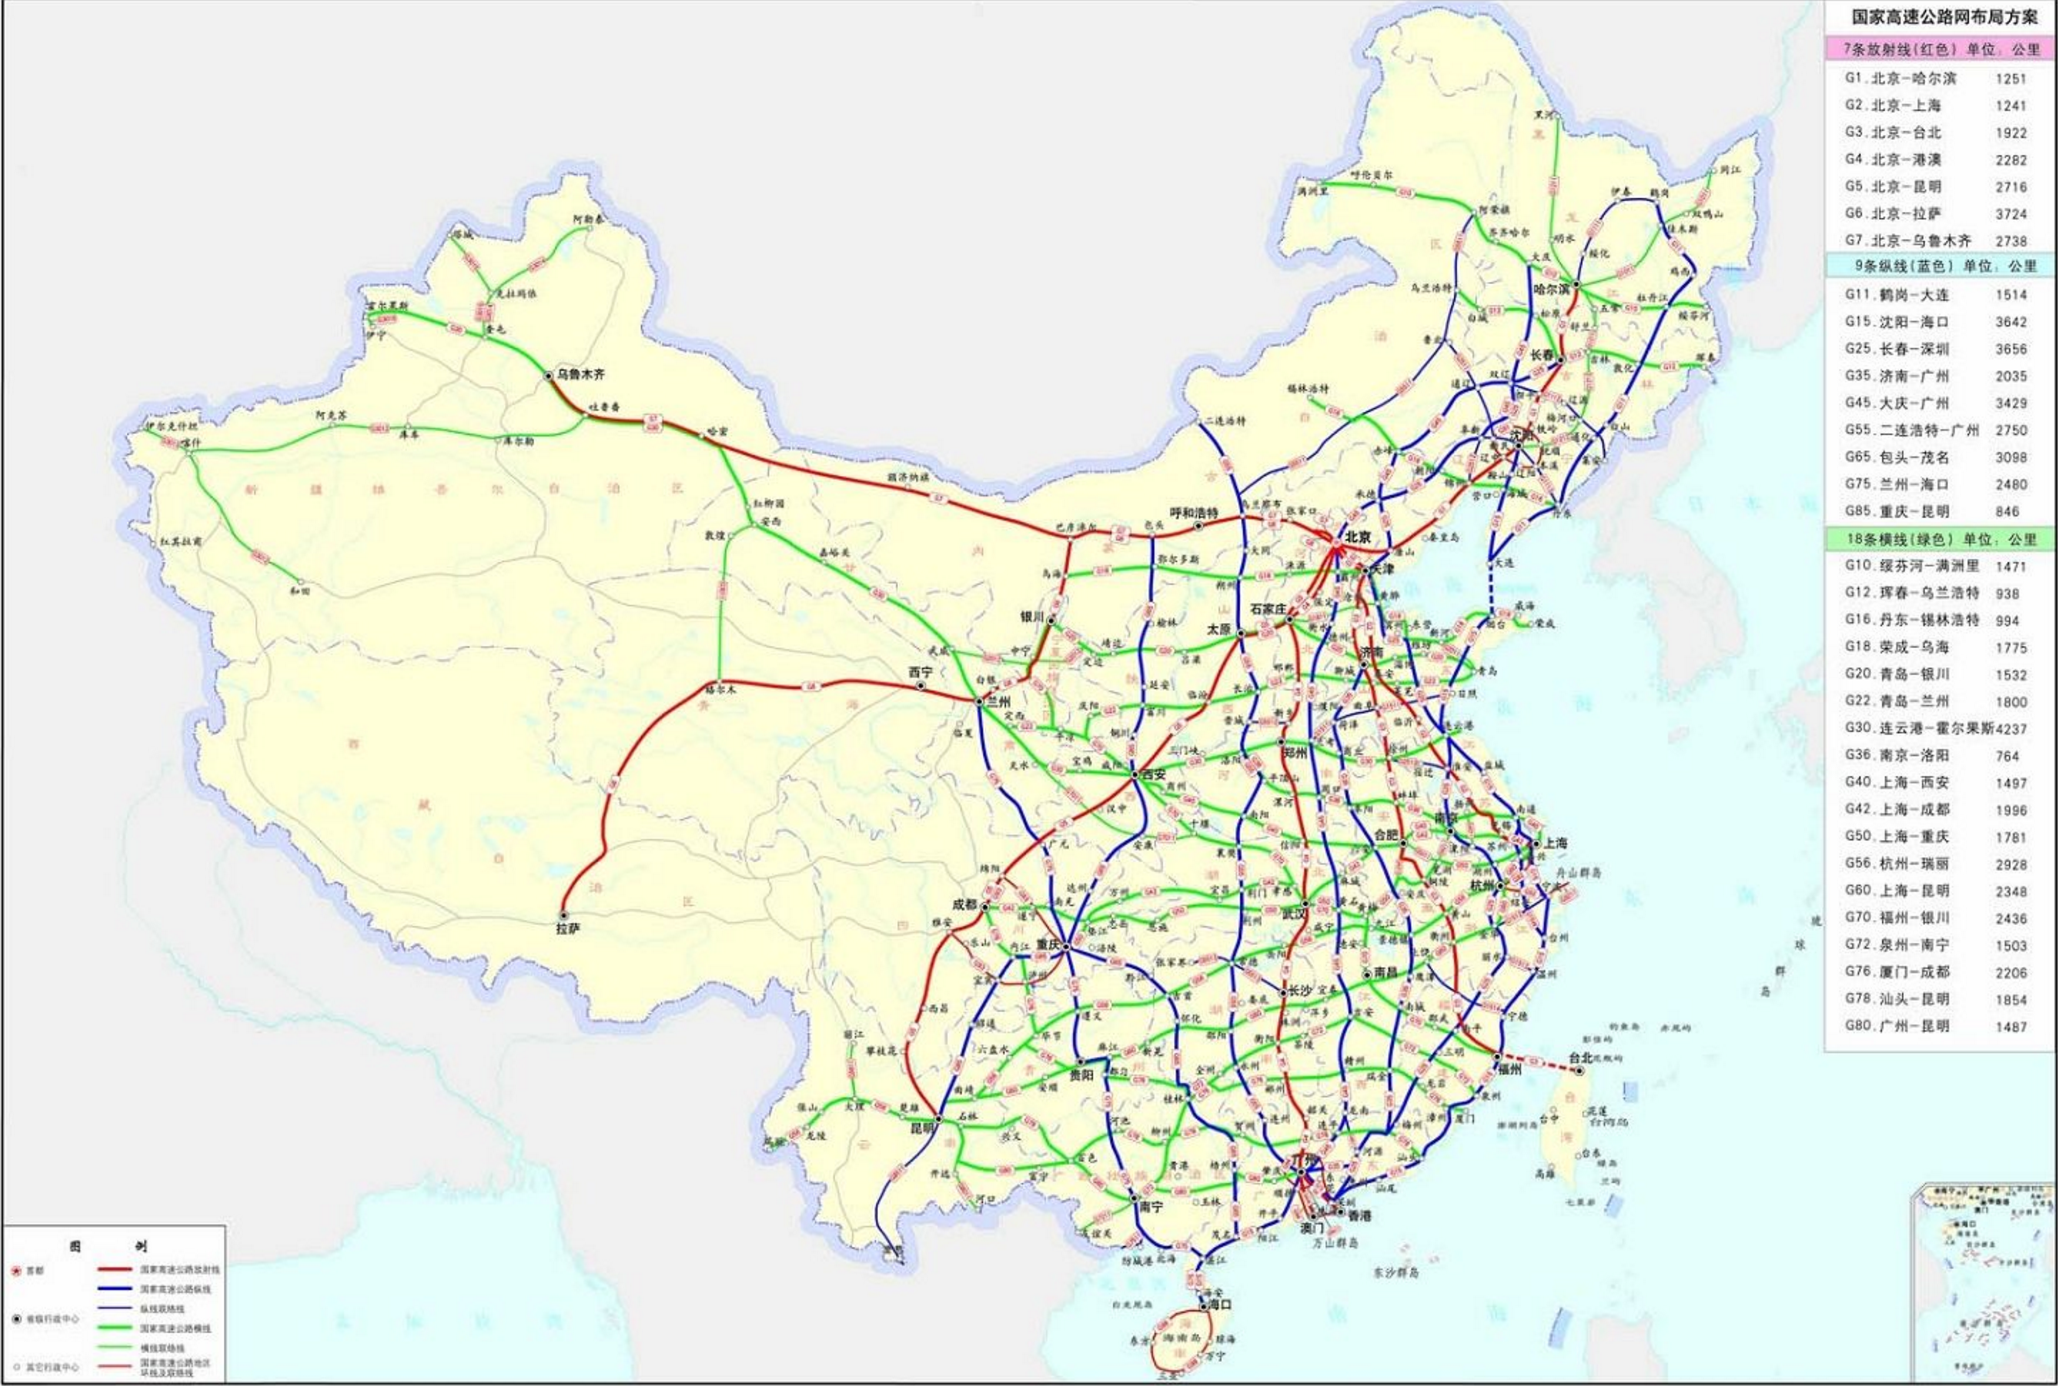
\includegraphics[width=4.4in]{picture/gaosugonglu}
							\caption{中国高速公路网络}
							\label{gaosugonglu}
						\end{minipage}%\
				\end{figure}

随着中国经济的快速发展,人们生活水平的不断提高,居民的出行和货物运输的数量也在逐渐增加。交通系统是人类活动不可缺少的一部分。据估计,每天平均有40\%的人口在路上花费至少1小时。近几年来,人们变得越来越依赖于交通系统,对于交通系统管理人员来说,机遇和挑战共存。首先,交通拥堵已成为一个日益严重的问题。全球范围内的道路上的车辆增加,根据调查,截止至2016年初,北京共有544万辆车,比2014年初增加了50万辆。这些激增的车辆会对道路系统产生严重的压力,极大的增加拥堵以及拥堵后的损耗。拥堵会导致燃油消耗增加,空气污染,以及实施公共交通计划的困难。车流流量过多时,交通事故风险与交通运输系统中的膨胀增加,交通事故之后的恢复时间与恢复代价也会急剧增加。在中国,2009年的交通事故死亡人数约有7万人,在2015年达到9万人。美国联邦公路管理局公布的报告显示,发生在城市的交通事故约占所有拥堵延误的50\% - 60\%。毫无疑问,如何高效处理交通事故和预测事故发生点,一旦世故发生,最大限度地减少其影响是一个核心问题。由于资源相对有限,尤其是中国高速公路正在逐渐走向免费,因此很难有预算全面建立新的基础设施。同时,运输系统的有效性也越来越依赖于一个国家的处理紧急情况的能力(例如,大规模疏散和安全增强)。一个国家的技术竞争力,其经济实力和生产能力,在很大程度上取决于其交通系统性能。随着高速公路的不断发展,各类维护高速公路的需求也都被一一提出,示例如下:

1)人员分配。最典型的是今年五一,山东高速管理人员联合曲阜路政大队、济宁京台高速交警大队、项目部制定有针对性的应急预案,根据历史的交通信息,负责做好恶劣天气、旅游高峰车流量饱和、突发事件引起交通阻塞的应急处理。安排值班人员,落实机械设备和应急物资准备,一旦发生突发事件,迅速启动,切实做好节日期的保畅工作。

2)安全管理。面对节日期间可能出现的状况,高速公路养护所需要在节日前期组织开展道路安全隐患检查活动:一是对管段路段进行安全隐患排查,发现问题立即落实整改;二是加强春季防火工作的管理,及时清理桥涵构造物下的易燃物品,对边坡、中央分隔带进行打草、苗木修剪,对匝道圈进行专人看护,安排养护员负责所辖路段的防火报警工作。

3)基础设施建设。交通的基础设施建设主要包括交通轨道交通设施建设、停车场设施建设等。交通基础设施包括为交通系统保障安全正常运营而建设的公路、轨道、隧道、高架道路、车站、通风亭、机电设备、供电系统、通信信号、道路标线等设施。

4)高新设施建设。目前越来越多的新技术涌现,比如说最近成都绕城高速公路的部分路段的养护施工采用了新技术——“就地热再生”。这是目前国际上先进的沥青路面施工技术,具有高效、优质、环保、节约的特点,施工过程中采用的是单车道施工方式,施工时占用的工作面小,不中断交通,施工完半小时路面温度降至50摄氏度即快速开放交通。同时就地热再生施工相比传统工艺,在温室气体排放量方面,每施工1万平方米可减少二氧化碳排放26吨,在资源的利用率方面,每施工1万平方米利用废旧沥青混合料960吨,节约新沥青料600吨。就地热再生方法在节能环保、废旧沥青再利用方面的优势在本次绕城高速施工中显现。

上述需求中有一个共性的问题,那就是如何找出高速公路网络中最重要的路段,然后针对这些重要路段,进行针对性管理。高速公路的变化日新月异,根据经验很难非常准确的预估出所有关键路段。亟需提出一套适用于大规模路网的高速公路的关键路段挖掘识别系统。在识别高速公路网络中关键路段的前提下,我们可以进行有效的人员分配,避免人员浪费;可以针对高危路段进行安全管理,减少事故风险;可以针对具有强烈需求的路段进行基础设施建设,避免资源浪费,也可以研究当关键路段因为施工等原因停滞时,如何将影响减少到最小。

本文提出的面向高速公路的关键路段挖掘模型就是一种为了满足上述需求而提出的模型。本文将重点分析高速公路网络的网络特点,以路段/网络运行效率模型为评价标准,在宏观层面上提出一种高速公路重要节点的挖掘模型,同时分析其模型性质,提出一种优化策略。从整体路网的流量角度提出适用于中国高速公路的大规模高速公路网络的关键路段识别算法。

本文针对高速公路进行关键路段挖掘,主要基于高速公路收费数据,并得到如下项目的支持:

1)山西/安徽省智能交通系统

	实验室曾经开发过面向山西/安徽省的智能交通系统,在这个系统里,我们开发了比较完善的底层数据存取框架,采用mysql数据库加infobright数据仓库的数据存储格式,Linq to sql数据存取方式,集成数据存取逻辑接口,为本研究提供数据基础。

2)国家科技支撑计划:高速公路网运行状态智能检测与安全服务保障关键技术研发及系统集成
	

				\begin{figure}[h]
				\centering
						\begin{minipage}{0.8\linewidth}
							\centering
							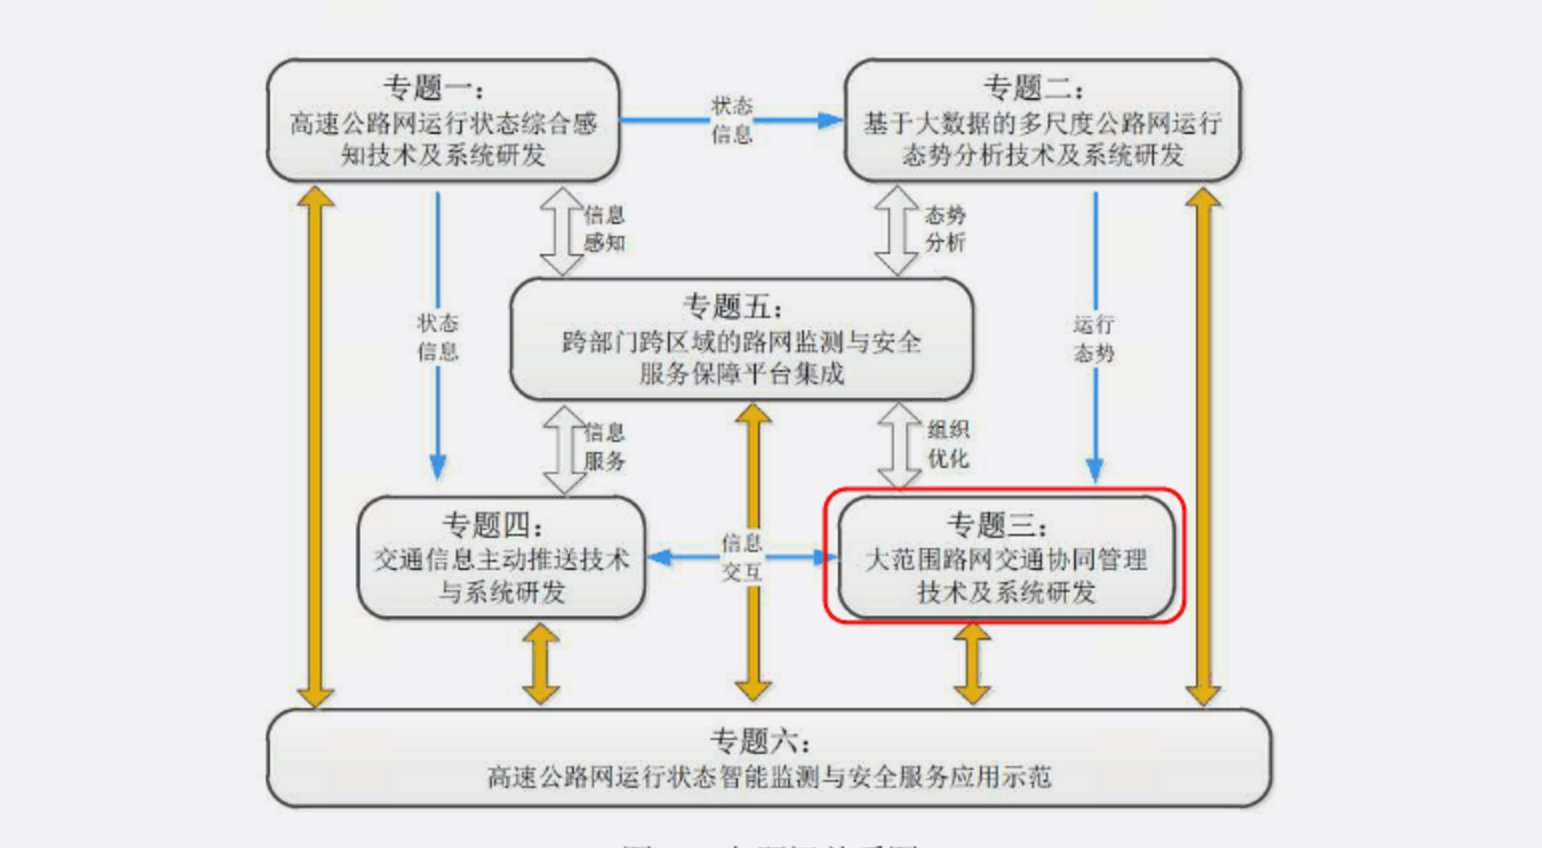
\includegraphics[width=4.4in]{picture/zhichengjihua}
							\caption{国家科技支撑计划}
							\label{zhichengjihua}
						\end{minipage}%\
				\end{figure}
图\ref{zhichengjihua}为项目专题间关系图,我们主要负责专题三:大范围路网交通协同管理技术以及系统研发。专题一主要研究高速公路的网络监测设施的部署问题,这些设施将用于改善路网运行状态以及获取路网运行数据;专题二主要用于分析和处理这些数据,将这些数据转化为流量、速度、密度和O-D信息。专题三负责提出决策模型,基于前面专题获取的数据,输出目前路网状态下最合理的绕行路线和限流建议;专题四负责研究如何设置设施,将这些建议分发出去;专题五和专题六负责将整个系统进行集成。可以看出,本课题中的专题一、专题三、专题四都和高速公路重要路段挖掘方法有关:专题一中的监测设施可以着重部署在重要路段中,以达到最大化优化监测数据的目的;专题三中的决策模型也可以基于路段的重要程度,采用弃小保大的策略,进行导流决策;专题四中可以根据重要路段的分布信息,划定信息发布点,优化信息发布行为。





\section{研究内容}
    本文从交通实际问题的角度出发,将一些具实际问题抽取共性,转化为通用的高速公路网关键路段挖掘问题。针对现有复杂网络关键路段挖掘技术的不足,提出以下两个研究内容:
    
		(1)提出一种度量高速公路节点重要性的研究模型。不管是在高速公路网上建设基础设施,还是部署警力,还是增加维护成本,都可以归类于对高速公路中路段的投资。本研究将其模型化,以每条路段都具有一定的损毁概率为基础,定义投资后路段的损毁概率下降。结合围观的路段概率矩阵,提出针对整体路网通行效率的宏观高速公路关键路段挖掘模型。并且分析模型的性质,给出贪心可解证明。可以在宏观层面反映这些节点对高速公路网络的影响,挖掘高速公路关键路段
		
		(2)提出一种结合高速公路网络特性的社群划分算法。关键路段挖掘模型本质上属于概率规划问题,时间复杂度达指数级。虽然在小范围路网中,计算时间少,静态关键路段的挖掘可以实现,但是在大范围路网中时间会巨额增长,直到不可忍受。同时因为算法需要时间较大,所以对于需要实时动态分析关键路段的需求无法满足。在分析了以往的模型求解方式不可解后,达到较强的收敛性与低误差。

\section{研究意义}
	本文研究工作的意义主要包括两个方面:

		1)应用实践价值:从应用的角度来看,随着我国高速公路网络规模的逐渐扩大,路网结构日益复杂,人们的出行需求逐年增加,高速公路遇到的挑战不断加大,高速公路的稳定越来越重要。同时随着高速监测设施的不断完善,可以实时监测高速公路中的车流信息,传统的研究方法中没有考虑关键路段会跟随流量和时间的变化而变化,本系统中加入考虑高速公路动态特性,优化时间复杂度,使得模型可以在可承受时间复杂度内求解,实现动态研究特性。

		2)理论研究价值:本文提出的面向高速公路的关键路段挖掘模型具有一定的理论创新性,他将一些高速公路建设上的具体问题抽象成一类问题,并给出一个可行解。传统高速公路关键路段研究,大多是研究高速公路的统计特性(如流量的大小,路段周围城市的重要程度,路段周围环境的变化等),本文利用数学模型描述各类高速公路现象,从宏观角度给出并求解一种具有普适性的高速公路关键路段挖掘模型。
		
\section{论文结构}
    第一章为绪论,介绍了本文的研究背景,提出了本文的研究内容。第二章
介绍了相关研究,主要介绍了高速公路关键路段研究、复杂网络关键路段研究的相关工作,结合交通问题的特点分析了现有方法的优势与不
足;同时对复杂网络社群划分方法及其相关研究进行了介绍,通过对现有社群划分方法的分类对比,分析了它们的优势与不足;第三章论述本
文的主要研究内容,提出了一种复杂网络关键路段挖掘模型,给出
了详尽的理论分析,并在多个数据集下进行了验证。第四章
提出了一种基于高速公路交通网络的社群划分模型,给出了高效的优化算法和详
尽的理论分析,并在多个数据集下的进行了验证。第五章给出了本文实现的一个原型系统,并且已经在实际数据上运行。第六章给出了全文的总结与未来工作展望。


